\chapter{The Dataset}
    %
    \begin{maxipage}
    \begin{bclogo}[couleur = vlightgray, logo = \bcinfo] {Recap}
    In the previous chapter, we set up our machine so that it has all of the software BioPype needs in order to function. \newline \newline In this chapter, we will use BioPype to \textbf{download} experimental data, and then prepare them for analysis via a process called \textbf{"quality control"}. We will also discuss how the BioPype functions used in this workflow were created.
    \end{bclogo}
    \end{maxipage}
    %

As described in Chapter \ref{chap:scene}, we want to investigate if there are any differences in the gut microbiomes of younger patients with IBD compared to older patients with IBD. Using the methods described in Chapter \ref{chap:find-tools}, we found a study in the SRA database with sequencing data that are useful to us. The webpage for the SRA Study is reproduced in Figure \ref{fig:ncbi-sra-study-page} and can be accessed at
    \url{https://trace.ncbi.nlm.nih.gov/Traces/sra/?study=SRP115494} .
    
%
\begin{figure}[hbtp]
    \begin{maxipage}
    \hrule
    \centering
    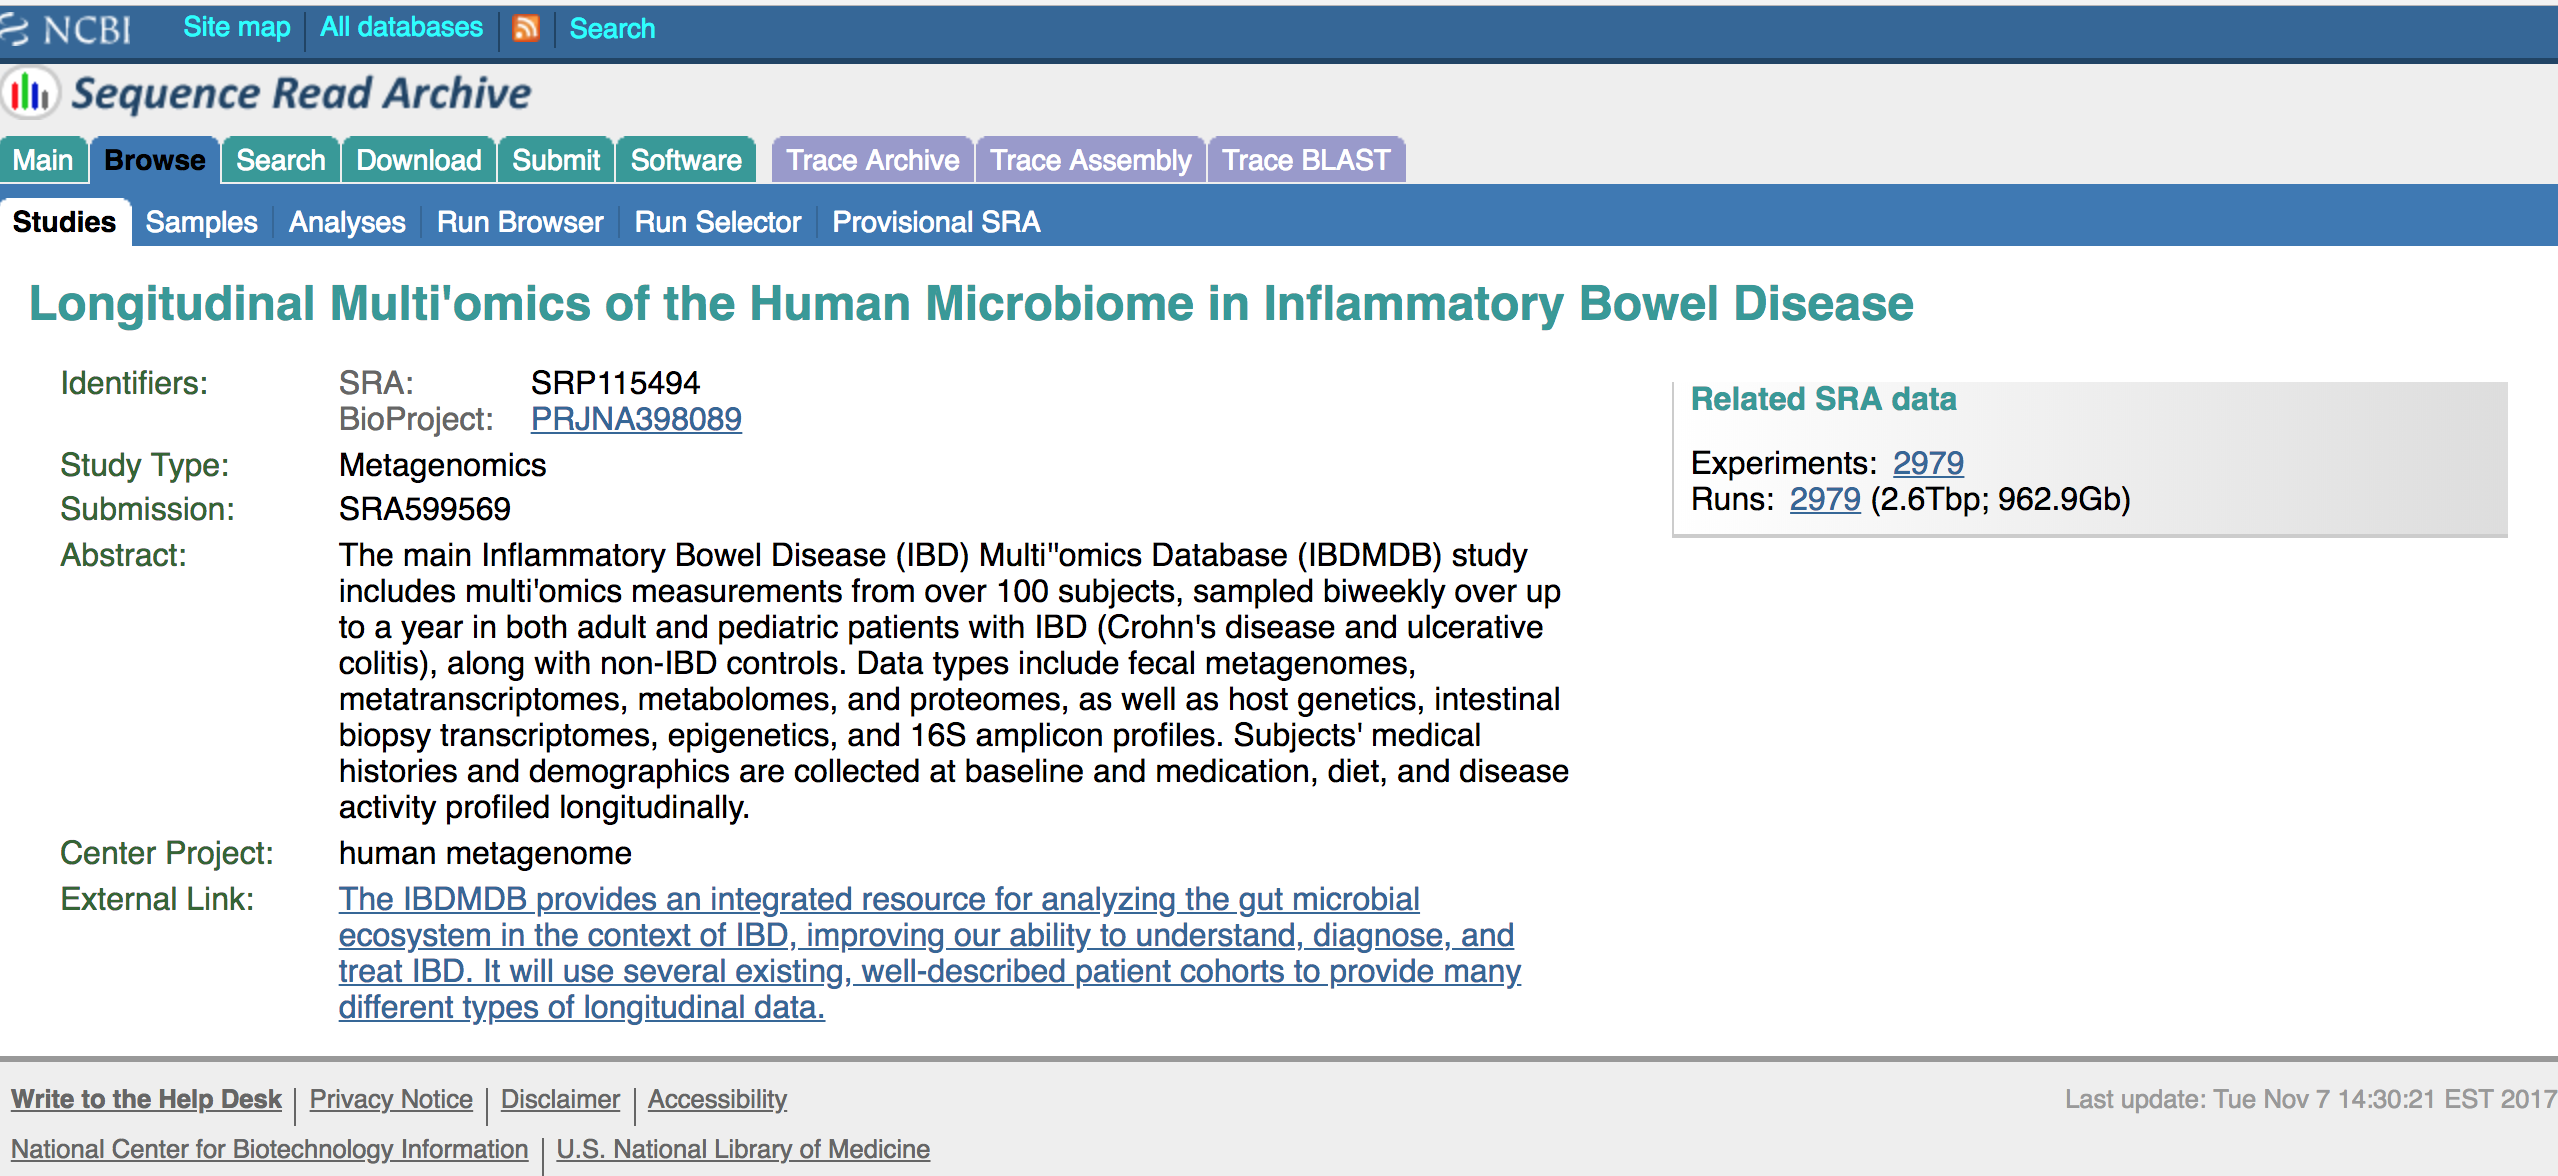
\includegraphics[height=8.75cm, width=16cm]{ncbi-sra-study-page}
    \caption{The "SRA Study" webpage.}
    \label{fig:ncbi-sra-study-page}
    \hrule
    \end{maxipage}
\end{figure}
%

The dataset is reproduced in Figure \ref{fig:ncbi-sra-runs-page} and can be found by clicking on "Runs" under "Related SRA data" on the right side of the SRA Study webpage, or by going to \url{https://trace.ncbi.nlm.nih.gov/Traces/study/?acc=SRP115494#} .

%
\begin{figure}[hbtp]
    \begin{maxipage}
    %\begin{center}
    \centering
    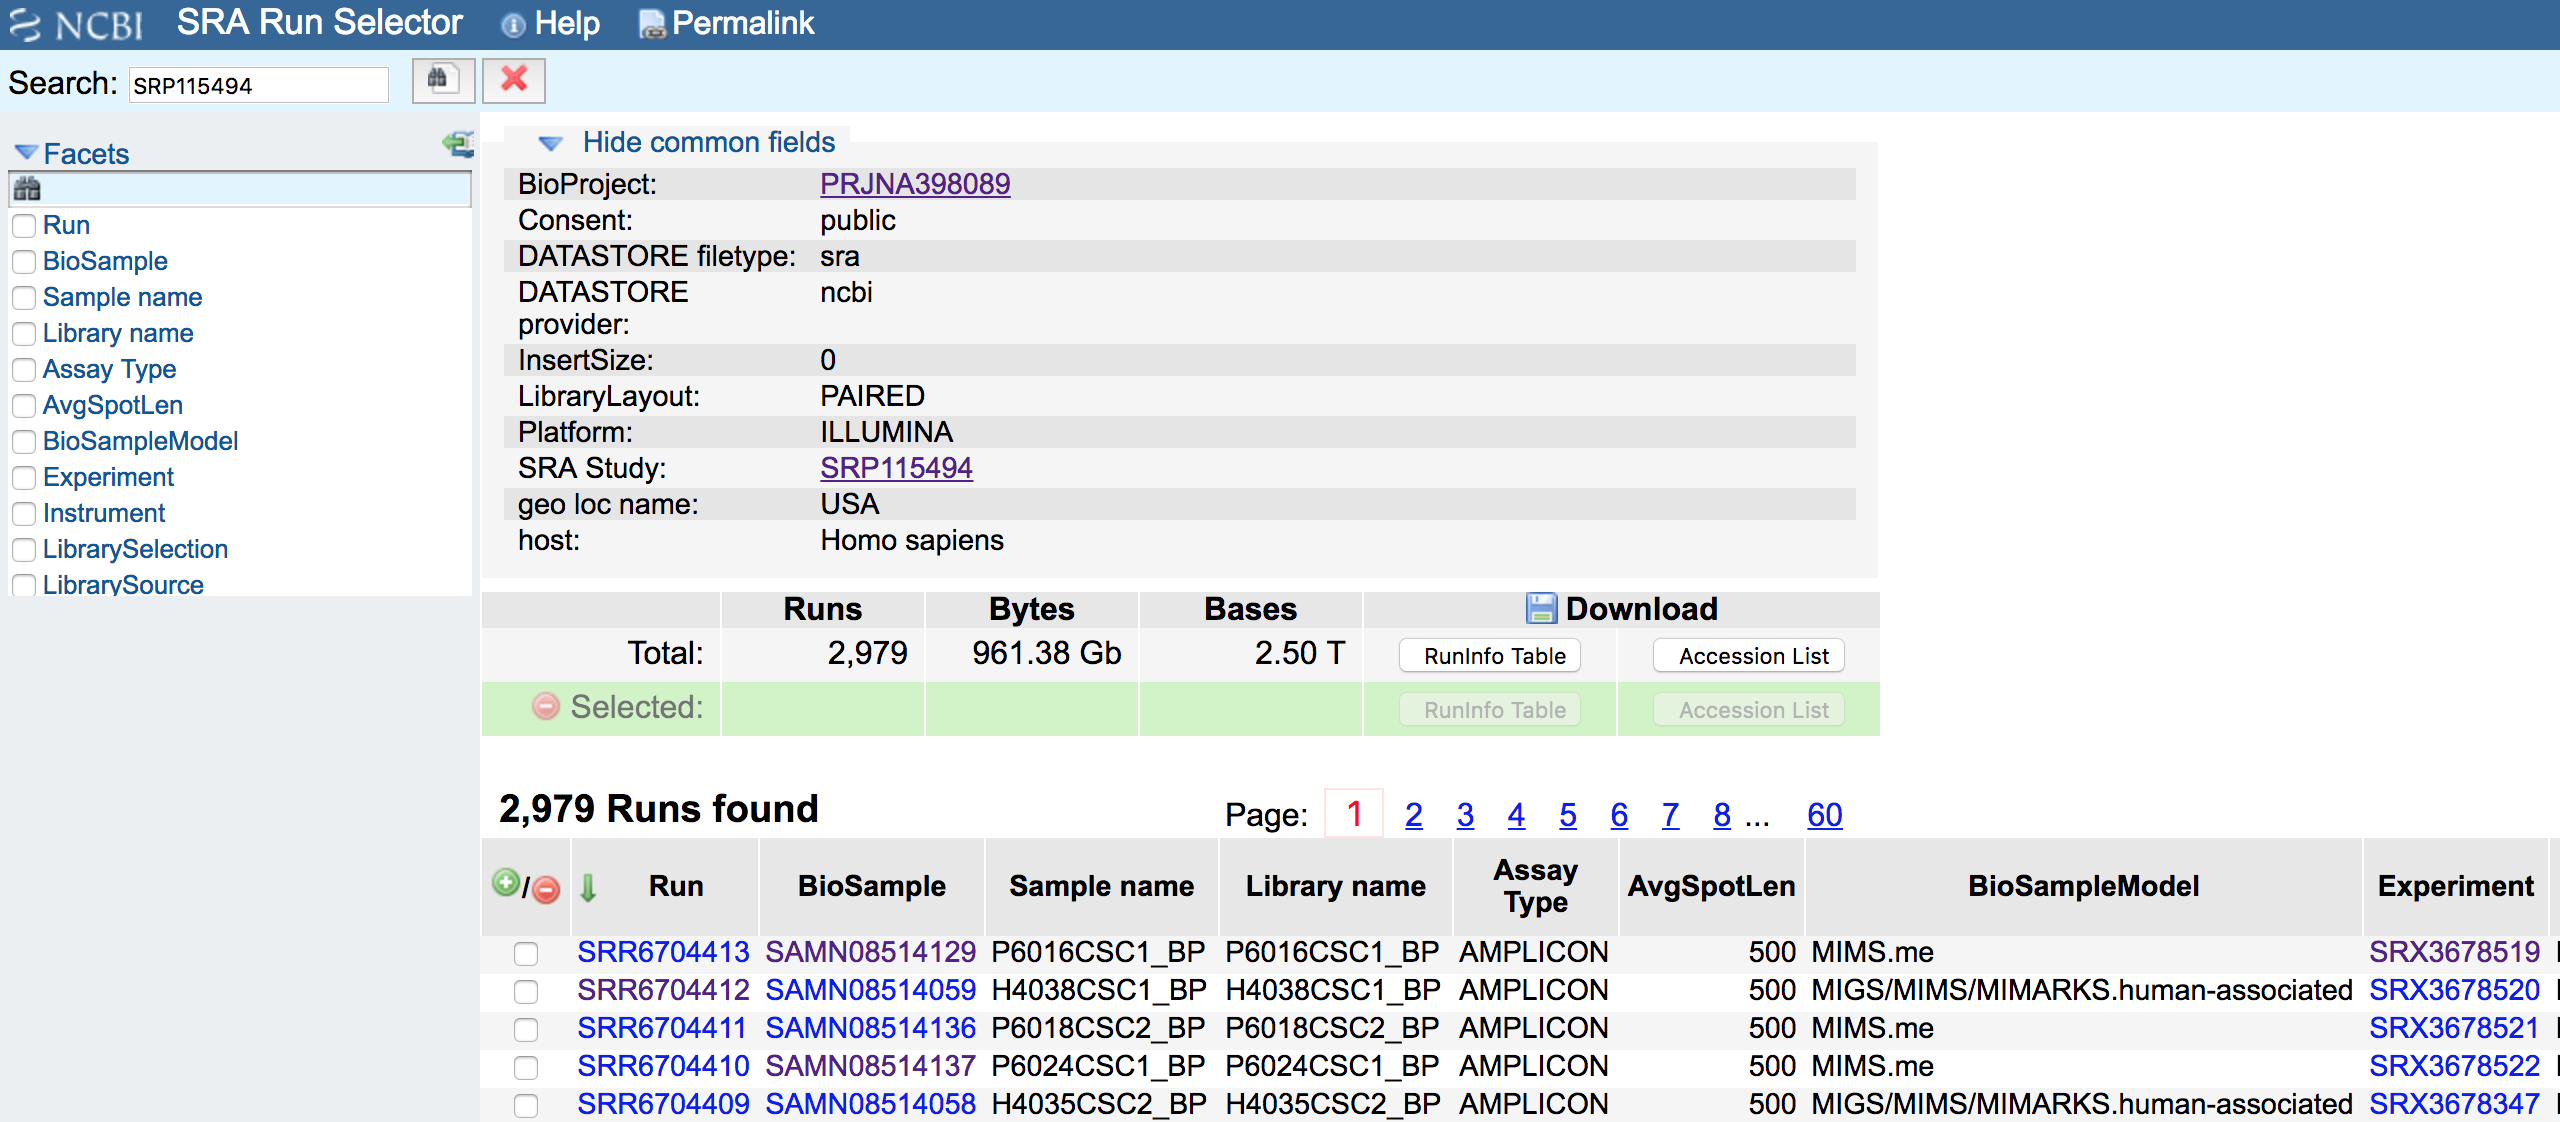
\includegraphics[height=8.5cm, width=16cm]{ncbi-sra-runs-page}
    \caption{The sequencing data collected by the \textit{Longitudinal Multi'omics of the Human Microbiome in Inflammatory Bowel Disease} study. (Note: the table's columns extend beyond the right side of the page because there are 36 metadata categories.)}
    \label{fig:ncbi-sra-runs-page}
    %\end{center}
    \end{maxipage}
\end{figure}
%
    
To learn more about how to use these pages to find information about the study and its methods, please refer to Chapter \ref{chap:find-tools}. 
    
    %
    \section{Download Dataset}
    
        \begin{enumerate}
            \item First, we must decide what criteria we will use to choose our experimental samples. 
            \marginlabel{Note: The dataset has a metadata category called "BioSample." This is not to be confused with the generic term "samples." In this case, one sample is equivalent to one run (i.e., one row) of the data table.}
            \newline
            Remember: our research question investigates the effects of age on the gut microbiomes of inflammatory bowel disease patients. Looking at the study abstract from Figure \ref{fig:ncbi-sra-study-page}, we can see that the researchers investigated two types of IBD: Crohn's disease and ulcerative colitis. So one of the metadata categories from the dataset (i.e., the columns from the dataset in Figure \ref{fig:ncbi-sra-runs-page}) that we will use to select our samples is the "host\_disease" category. We will also select our samples based on the "host\_age" metadata. Finally, our relative abundance analysis will require amplicon sequencing data, so the third metadata category we will sort by is the "Assay\_Type" column.
            
            \item Now we want to select our samples based on these categories. 
            
            Download the RunInfo Table file found on the study's sample page and put it in the project folder you set up in Chapter \ref{software}. The RunInfo table is just the browser's sample table in a .txt file format.
            
            \item Open the command line interface for your machine's operating system. On a mac, this is the Terminal application. 
            
            \item Navigate to your project's folder and then confirm that you are in the right location by using the the following commands at the command prompt:
            
                \begin{lstlisting} [language=Python]
$ cd <path_to_your_project>
$ pwd
                \end{lstlisting}
                        
            \item Activate the Python interpreter by typing the following into the command prompt:
                \begin{lstlisting} [language=Python]
$ python3
                \end{lstlisting}
            
            \item Import BioPype to the current Python environment:
                \begin{lstlisting} [language=Python]
>>> import BioPype
                \end{lstlisting}
                
                    \begin{itemize}
                    \item \attention{If not done already, stop and follow the instructions in Chapter \ref{chap:software} to configure the BioPype working directory and the SRA Toolkit Workspace Location.}
                    \end{itemize}
                
            \item Import \verb|BioPype.cmds.runtable| to gain access to the \verb|RunTable| class:
            \marginlabel{\footnotesize Using "as" in an import statement lets you reference the full name of the imported package by some shorter name. It is generally considered better practice to \textbf{not} import packages "as" some other name, because it makes the code less explicit (which goes against the purpose of Python), but we do it in this manual for the sake of space.}
                \begin{lstlisting} [basicstyle=\small, language=Python]
>>> import BioPype.cmds.runtable as rt
                \end{lstlisting}
                
            \item Import the rest of the Python packages that we will need for the analysis:
            \begin{lstlisting} [basicstyle=\small, language=Python]
>>>import os
>>>import glob
>>>import pandas as pd
>>>from BioPype.cmds.downloadsra import DownloadHelper
            \end{lstlisting}
                
            \item Create a \verb|RunTable| object called "my\_table" out of the RunInfo Table .txt file:
            \begin{lstlisting} [basicstyle=\footnotesize, language=Python]
>>> my_table = rt.RunTable('runinfotable_filename.txt')
            \end{lstlisting}
            
            
                \begin{itemize}
                \item With the \verb|my_table| object created, you can remind yourself what the metadata categories are by using the following command:
                \end{itemize}
                \begin{lstlisting} [basicstyle=\footnotesize, language=Python]
>>> my_table.column_names
['Assay_Type', 'AvgSpotLen', 'BioSample', 'BioSampleModel', 
 'Experiment', 'Instrument', 'LibrarySelection', 'LibrarySource', 
 'Library_Name', 'LoadDate', 'MBases', 'MBytes', 'Organism', 
 'ReleaseDate', 'Run', 'SRA_Sample', 'Sample_Name', 
 'collection_date', 'env_biome', 'env_feature', 'env_material', 
 'host_age', 'host_disease', 'host_sex', 'host_subject_id', 
 'lat_lon', 'BioProject', 'Consent', 'DATASTORE_filetype', 
 'DATASTORE_provider', 'InsertSize', 'LibraryLayout', 'Platform', 
 'SRA_Study', 'geo_loc_name', 'host']
                \end{lstlisting}
                
                
            \item We want to first group the samples based on whether they contain amplicon sequencing data instead of whole genome sequencing data...
             \begin{lstlisting} [basicstyle=\scriptsize, language=Python]
>>>amp_samples = my_table.filter_data("Assay_Type", '==', 'AMPLICON')
            \end{lstlisting}
            
            \item We then want to group the samples based on the patients' condition...
            \begin{lstlisting} [basicstyle=\scriptsize, language=Python]
>>>uc_samples=amp_samples.filter_data("host_disease", '==', 'UC')
>>>cd_samples=amp_samples.filter_data("host_disease", '==', 'CD')
            \end{lstlisting}
            
                
            \item ... then we want to group them based on age:
            \begin{lstlisting} [basicstyle=\small, language=Python]
>>>uc_young = uc_samples.filter_data("host_age", '<=', 21)
>>>uc_old = uc_samples.filter_data("host_age", '>=', 40)
>>>cd_young = cd_samples.filter_data("host_age", '<=', 21)
>>>cd_old = cd_samples.filter_data("host_age", '>=', 40)
            \end{lstlisting}
                \begin{itemize}
                \item \attention{Note} that the third argument passed to the \verb|filter_data()| method is \textbf{not} a string like the previous two arguments. It is simply an integer (no quotation marks around it).
                \end{itemize}
                
                
            \item Now that we have groups of samples selected, we want to get a list of SRA accession numbers for each group. The accession numbers are what we will use to specify the files we want to download from the SRA database. 
            \begin{lstlisting} [basicstyle=\small, language=Python]
>>>uc_young_nums = uc_young.get_accession_numbers()
>>>uc_old_nums = uc_old.get_accession_numbers()
>>>cd_young_nums = cd_young.get_accession_numbers()
>>>cd_old_nums = cd_old.get_accession_numbers()
            \end{lstlisting}
            
%             
            \item To handle the process of downloading the .sra files from the SRA database, we instantiate 'DownloadHelper' objects: 
            \begin{lstlisting} [basicstyle=\footnotesize, language=Python]
>>>uc_young_obj = DownloadHelper(uc_young_nums, 5, threads=4)
>>>uc_old_obj = DownloadHelper(uc_old_nums, 5, threads=4)
>>>cd_young_obj = DownloadHelper(cd_young_nums, 5, threads=4)
>>>cd_old_obj = DownloadHelper(cd_old_nums, 5, threads=4)
\end{lstlisting}

            Three arguments are passed to the objects when they're created:
            \begin{enumerate}
	       \item A list of accession numbers
	       \item The number of samples we want to randomly select from the list of accession numbers. To account for hardware limitations that would severely bottleneck the analysis at file-handling steps like these, we will randomly select a subset of only 5 accession numbers
	       \item \seealso{To learn more about what threads are, and how many you should use, see Appendix \ref{app:threads}.} The number of threads we want our computer to use while handling the download and conversion of .sra files to .fastq files.
            \end{enumerate}
            
            \begin{itemize}
	   \item The more threads your computer can divide this process between, the better (it's more complicated than that, but for now let's go with it). The question is: how many threads is your computer capable of using? For that, you'll have to do some Googling. You can find the resources I used to figure out how many threads my MacBook Pro can run (4) in Appendix \ref{app:threads-resources}. To simplify: my computer has 1 CPU, the CPU has 2 cores, and each core can run 2 threads. 1 x 2 x 2 = 4 threads.
	   \end{itemize}
%            
            
            \item \seealso{To learn more about .sra file format, see Appendix \ref{app:sra-format}.} We can now download the SRA files and convert them to FASTQ format:
            \seealso{To learn more about .fastq format, see Appendix \ref{app:fastq-format}.}
            \begin{lstlisting} [basicstyle=\footnotesize, language=Python]
>>>uc_young_obj.download_paired_end_data('uc_young', 'uc_young')
>>>uc_old_obj.download_paired_end_data('uc_old', 'uc_old')
>>>cd_young_obj.download_paired_end_data('cd_young', 'cd_young')
>>>cd_old_obj.download_paired_end_data('cd_old', 'cd_old')
            \end{lstlisting}
            \marginlabel{The .sra files will not be downloaded to the correct location if the SRA Toolkit Workspace Location has not been properly configured (see Chapter \ref{chap:software} for details)} Here, we are using the \verb|.download_paired_end_data()| class method, which takes two arguments:
            \begin{enumerate}
            \item The name of the folder which will contain the downloaded .sra files for an experimental group, and that will be saved inside the "data.grouped\_sra" directory in the SRA Workspace (e.g., we want the .sra files for the "Crohn's-Disease-Younger" experimental group to be saved to the \newline "biopype\_project/data/grouped\_sra/cd\_young" directory).
            \item The name of the folder which will contain the downloaded .fastq files for an experimental group, and that will be saved inside the "data.grouped\_fastq" directory in the SRA Workspace (e.g., we want the .fastq files for the "Crohn's-Disease-Younger" experimental group to be saved to the \newline "biopype\_project/data/grouped\_fastq/cd\_young" directory).
            \end{enumerate}
            
        \end{enumerate}
        
After this last step, we will have downloaded all of our experimental samples and converted them from .sra files to .fastq files! Next, we will perform quality control on the dataset, then perform the relative abundance analysis.
                
        %
    
    
    \section{Perform Quality Control on Dataset}

